% プロジェクト学習中間報告書書式テンプレート ver.1.0 (utf-8)

% 両面印刷する場合は `openany' を削除する
\documentclass[openany,11pt,papersize,dvipdfm]{jsbook}

% 報告書提出用スタイルファイル
%\usepackage[final]{funpro}%最終報告書
\usepackage[middle]{funpro}%中間報告書

% 画像ファイル (EPS, EPDF, PNG) を読み込むために
\usepackage{graphicx}

\usepackage{float}

\def\hissu{\bgroup\color{red}}
\def\endhissu{\egroup}

% ここから -->
%\usepackage{calc,ifthen}
%\newcounter{hoge}
%\newcommand{\fake}[1]{\whiledo{\thehoge<70}{#1\stepcounter{hoge}}%
%  \setcounter{hoge}{0}}
% <-- ここまで 削除してもよい

% 年度の指定
\thisYear{2023}

% プロジェクト名
\jProjectName{使ってもらって学ぶフィールド指向システムデザイン~2023}

% [簡易版のプロジェクト名]{正式なプロジェクト名}
% 欧文のプロジェクト名が極端に長い（2行を超える）場合は，短い記述を
% 任意引数として渡す．
%\eProjectName[Making Delicious curry]{How to make delicious curry of Hakodate}
\eProjectName{Field~Oriented~System~Design~Learning~by~Users'~Feedback~2023}

% <プロジェクト番号>-<グループ名>
\ProjectNumber{3-C}

% グループ名
\jGroupName{グループ~C（未来大生支援）}
\eGroupName{Group~C~(FUN Student Support)}

% プロジェクトリーダ      注意：学籍番号不用
\ProjectLeader{佐々木虎太郎}{Kotaro~Sasaki}

% グループリーダ      注意：学籍番号不用
\GroupLeader  {大須賀雅也}{Masaya~Osuga}

% メンバー数
\SumOfMembers{9}
% グループメンバ      注意：学籍番号不用
\GroupMember  {1}{大須賀雅也}{Masaya~Osuga}
\GroupMember  {2}{齊藤輝}{Hikaru~Saitou}
\GroupMember  {3}{南川虎之介}{Toranosuke~Minamikawa}
\GroupMember  {4}{鈴木利芳}{Masayoshi~Suzuki}
\GroupMember  {5}{高橋慧流}{Satoru~Takahashi}



% 指導教員
\jadvisor{伊藤恵,南部美砂子,奥野拓,元木環,石尾隆}
% 複数人数いる場合はカンマ(,)で区切る．カンマの前後に空白は入れない．
\eadvisor{Kei~Ito,Misako~Nambu,Taku~Okuno,Tamaki~Motoki,Takashi~Isio}

% 論文提出日
\jdate{2023年7月21日}
\edate{July~21, 2023}

\begin{document}
%
% 表紙
\maketitle

%======================================================================
%前付け
\frontmatter

% 和文概要
\begin{jabstract}
本プロジェクトは，フィールド調査をもとに問題を発見し，ITを用いて解決する．それによりユーザの仕事や生活をデザインし，地域や社会に貢献することを目的に活動している．また，本プロジェクトは，アジャイル開発手法を用いる．それにより，迅速で柔軟な開発を行い，短期間の開発でより効率的に成果を出すことを目標にしている．今年度は，プロジェクト内を交通グループ，小学校支援グループ，未来大生支援グループの3グループに分け，各グループがそれぞれのフィールドで活動している．本報告では未来大生支援グループについての報告を行う．本グループでは，公立はこだて未来大学に在籍している学生に対し，情報を取得しやすくすることで学生生活を効率的に送れるよう支援することを目的として活動している．この目的を達成するため，私達が実際に生活しているうえで取得しにくい情報が何かを話し合い，周りの学生にもヒアリングを行った．その結果，「HOPEやSTUDENTSに情報が分散していて目的の情報が探しづらい」という問題点が挙がり，公立はこだて未来大学の情報を一元化したアプリを作成することに決定した．このプロダクトを提案することにより，学生が欲しい情報を簡単に見つけ出せる環境を実現し，学生生活の効率性を高めることを狙う．これまで，実現可能範囲を調査するための技術検証や既存サービスの調査を行ってきた．今後は，実装する機能を確定させ，開発に必要な技術を習得し取り組んでいく予定である．

% 和文キーワード
\begin{jkeyword}
フィールド調査，IT，スクラム，学生支援，情報一元化
\end{jkeyword}
\bunseki{齊藤輝}
\end{jabstract}

%英語の概要
\begin{eabstract} Abstract in English. 
This project identifies problems based on field research and solves them using IT. The
project design the work and life of users and contribute to the community and society through these activities. The project will use agile development methods. The goal is to develop quickly and flexibly, thereby achieving more efficient results in a short development period. This year, the project is divided into three development groups: a transportation support group, a local media group, and a local media group, with each group working in its own field. In this report, we report on the traffic support group. In this group, the purpose of this group is to support students enrolled at Future University Hakodate by facilitating access to information, thereby enabling them to lead a more efficient student life. To achieve this goal, we discussed the challenges of obtaining information in our daily lives and conducted interviews with fellow students. As a result, we identified the issue of scattered information across HOPE and STUDENT platforms, making it difficult to find specific information. To address this, we have decided to create an application that consolidates the information available at Future University Hakodate. By proposing this product, our aim is to create an environment where students can easily find the information they need, ultimately enhancing the efficiency of their student life. So far, we have conducted technical feasibility studies and examined existing services. Going forward, our plan is to determine the required features and acquire the necessary technology for development.







% 英文キーワード
\begin{ekeyword}
Field research, IT, Scrum, University Student Support, Centralized information
\end{ekeyword}
\bunseki{齊藤輝}
\end{eabstract}

\tableofcontents% 目次

%======================================================================
\mainmatter% 本文のはじまり

%各章の.texファイルをここに並べる
%ファイル名の「.tex」は省略して良い
\chapter{背景と目的}
%該当分野の従来の状況，問題点，本プロジェクトで設定した課題，実施した解決策，及び成果を簡潔に記述する．


\section{プロジェクトの立ち上げ}

世の中にはニーズを十分に満たしていないシステムが存在する．これは，開発者が作るものとユーザが求めるものとの乖離が原因の1つであると考えられる．この問題を解決するためには，ユーザを理解してシステムを開発する必要があることから，開発者が現場に赴き，調査をして，ユーザから直接学ぶべきであると考えた．そこで「使ってもらって学ぶフィールド指向システムデザイン」を理念とするプロジェクトが始まった．
\bunseki{大須賀雅也}

\section{プロジェクトの方針}
本プロジェクトは，例年実際に現場に赴くフィールド調査とアジャイル開発手法の1つである，スクラム手法\cite{scrumb}を採用している．フィールド調査ではユーザの思考や行動などの，現場に行かないと分からないことを知ることができる．また，スクラムは，アジャイル開発の中でも少人数のチームで開発を行い，スプリントと呼ばれる固定の短い時間に区切って作業を進めるものである\cite{scrumb}．これはユーザのフィードバックを繰り返し受けて，改善する機会を何度も得ることができるため，本プロジェクトの「使ってもらって学ぶフィールド指向システムデザイン」という理念と合致する．以上のことから，今年度もフィールド調査とスクラム手法を採用することにした．
\bunseki{大須賀雅也}

\section{未来大生支援グループ}\label{sec:gaiyou}
% 上述の問題点を解決すべく当プロジェクトの掲げる課題の概要を述べる．
私達未来大生支援グループは初め，函館市の病院に関連するアプリを開発することを目的として結成された．病院に関連するアプリについてアイディアを出す過程で，課題に対する具体的なアイディアが出尽くしたと感じ，このままでは興味深い結果が得られないと考えるようになった．この状況を受け，一度全てを白紙に戻し，全体を再度検討することとした．そして，私達自身に有用なアプリの開発に焦点を当てることを決定した．私達全員が日常的に利用し，かつ改善の余地があると感じるものを対象に検討した結果，私たち自身が在籍する公立はこだて未来大学に注目することとなった．普段から大学のシステムを頻繁に利用している私達は，その操作性の悪さに共通認識を持っていた．この認識を背景に，再度ブレインストーミングを行った．その結果，大学のシステムを単に改善するだけでなく，大学生活の利便性を高めることを目指すことになった．具体的には，私達が抱える問題を解決するため，公立はこだて未来大学の情報を一元化したアプリを開発することを決定した．

\bunseki{大須賀雅也}

\chapter{前期の主な活動}
私達大学グループは，当初病院グループとして結成された．函館市の病院に関連するサービスを作ることで，病院を利用する際の利便性を高めようとすることが目的のグループである．

\bunseki{大須賀雅也}

\section{病院グループとしての活動}

\subsection{既存のサービスの調査}
私達は，5月24日のグループワークで，函館に存在する病院関連サービスの問題点と良い点を調査した．はこだて医療情報\footnote{http://www.medical-h.net}というWebサイトとGrucco\footnote{https://www.city.hakodate.hokkaido.jp/docs/2017051700047/}というモバイルアプリを調査の対象とした．グループの全員でそれぞれのサービスに実際に触れてみた．触れた結果挙がった感想を以下に記述する．
\vskip\baselineskip

\begin{description}
\item[はこだて医療情報] \mbox{} \\\\
良いところ
\\
\begin{itemize}
\item 情報が網羅されていそう
\item 検索は意外とできそう
\item 詳しくのっていそう
\end{itemize}
\mbox{} \\
悪いところ
\\
\begin{itemize}
\item 使いにくい
\item 検索システムが見づらい
\item ダサい
\item 地図が使えない
\item 自分で入力して検索することができない
\item スマホでみにくい
\item 検索するのに時間がかかる
\item 情報が飽和していて必要な情報を選びづらい
\item 存在するはずの情報が存在しない
\item 古い
\end{itemize}

\end{description}

\clearpage
\begin{description}
\item[Grucco] \mbox{} \\\\
良いところ
\vskip\baselineskip
\begin{itemize}
\item 健診\item 予防接種のお知らせの通知設定ができる
\item 記事のお気に入り機能がある
\end{itemize}
\mbox{} \\
悪いところ
\\\\
全体
\begin{itemize}
\item 最新Androidのバージョンに対応していない
\item 定期的にフッターメニュー押せなくなる
\item アイコンが各タブで統一されている→ホームの新着情報で区別できるけど
\end{itemize}
\mbox{} \\
ホーム
\begin{itemize}
\item 夜間急病センター案内へのリンク飛ばし
\item ジャンルの順番
\item こちらから検索，検索わかりにくい
\end{itemize}
\mbox{} \\
施設
\begin{itemize}
\item ジャンルによるピンに違いがない，全部これ
\item ジャンル複数選択できない
\item 病院というジャンルが存在しない
\end{itemize}
\mbox{} \\
イベント
\begin{itemize}
\item 日付の記載が日付欄とタイトル【】でばらばら
\item お知らせ
\item お気に入り
\item 施設ページから地図をみれない
\end{itemize}

\end{description}

\bunseki{大須賀雅也}

\subsection{ペルソナ分析}
TAの方から，対象者を考える時はペルソナを用いて考える事によって，グループメンバーが対象者を想像しやすくなるというご指摘を受けたため，グループメンバーでペルソナを考えることにした．ChatGPT\footnote{https://chat.openai.com/}を用いて，10代から80代までの存在しない人物のプロフィールを生成し，それぞれの人物が「どのような時に病院を利用するか」「なぜ病院を探すのか」について検討した．

\bunseki{大須賀雅也}

\section{テーマの変更}
%1.3節で述べた課題をより具体的に記述する．成果に対して必ず満たすべき条件を含む

私達は，5月31日に行ったグループワークで，それまでに検討していた病院に関連したアプリのアイディアに行き詰まり，次回までの宿題として「アプリを作る前提でのコンセプト」「方向性，機能」などをそれぞれ各自で考えてくることとした．そして，6月2日のグループワークで，それぞれの考えてきたことを発表しあった．その結果，自分たちが在籍している公立はこだて未来大学に関連するアプリを開発するという案が採用された．採用された理由は，公立はこだて未来大学は私達が在籍している大学であるため，存在する問題を詳しく理解している．加えて，存在する問題を解決することが私たちに直接役に立つため，以前の病院に関連したアプリ開発よりモチベーションが維持しやすいからである．


\bunseki{大須賀雅也}

\section{公立はこだて未来大学の問題点}
次に，公立はこだて未来大学に存在する問題について具体的に考えた．真っ先に挙げられた問題は，公立はこだて未来大学のシステムが使いにくいということであった．具体的には，「HOPE\footnote{https://hope.fun.ac.jp/}やSTUDENTS\footnote{https://students.fun.ac.jp}のどこにどの情報があるのかがわからない」や「情報がまとまっていない」などである．そしてHOPEやSTUDENTSのどういった情報が必要なのかを検討した．私たちが必要だと感じた情報として以下の様な案が挙げられた.
\begin{itemize}
      \item 単位にかかわる詳細情報
      \item 評価基準
      \item 授業フィードバック
      \item 課題に関する情報
      \item 先生方のメールアドレス
      \item 教室情報
\end{itemize}
これらの情報は，HOPEやSTUDENTSに存在するが探すのが面倒であったり，そもそもどこにあるかがわからないという問題があることが分かった．そのため，これらの情報をまとめるということが一つの課題となった．

\bunseki{大須賀雅也}

\section{プロダクトの考案}
次に，大学で生活するうえでどんなサービスが欲しいかについて意見を出し合いホワイトボードにアイディアを羅列していった．そこで，「学生間で不必要になったものなどをやり取りするもの（ジモティのようなもの）」「学内，学外アルバイト」「飲食店の情報」「料理の情報」「過去問」「テーブルの空きがわかるマップ」「課題の締め切り情報一覧」などの意見が出た．そして，ここまでで出たアイディアの中でどのサービスが一番欲しいかグループ内で投票をした．その結果「学生間で不必要になったものなどをやり取りするもの（ジモティのようなもの）」「過去問」「課題情報」「テーブルの空きがわかるマップ」が私たちが欲しているものだということが分かった．そこで，以下の四つの軸でアプリを開発することに決定した．
\begin{itemize}
      \item 情報系
      \item 学生間で不必要になったものなどをやり取りするもの（ジモティのようなもの）
      \item 授業系
      \item マップ系
\end{itemize}
そして，この四つの軸にどのような機能を実装するかホワイトボードに書き出してまとめる作業を行った．情報系は「バイト」「イベント」「過去問」「就活」などの情報を表示する．授業系は「課題締め切り」「授業フィードバック」「VEP関連」「単位情報」「評価基準」などの情報をまとめる．マップ系は「テーブルの空き」「教室の空き」「コンセントの場所」「部屋の名称」「気温や空調」などを表示する．「学生間で不必要になったものなどをやり取りするもの（ジモティのようなもの）」は教科書や家具や服や備品などをやり取りできるようにする．

\bunseki{大須賀雅也}

\section{ブレインストーミング}

ブレインストーミングはホワイトボードを使って行った（図\ref{fig:brain}）．グループのメンバーがそれぞれ思いついたアイディアを書いていくという形をとった．ブレインストーミングでは公立はこだて未来大学の問題だけではなく，あったらいいものや欲しいものなど様々なアイディアが挙げられた．ブレインストーミングにはTAの方にも協力していただき様々なアイディアやアドバイスを頂いた．
\begin{figure}[H]
    \centering
    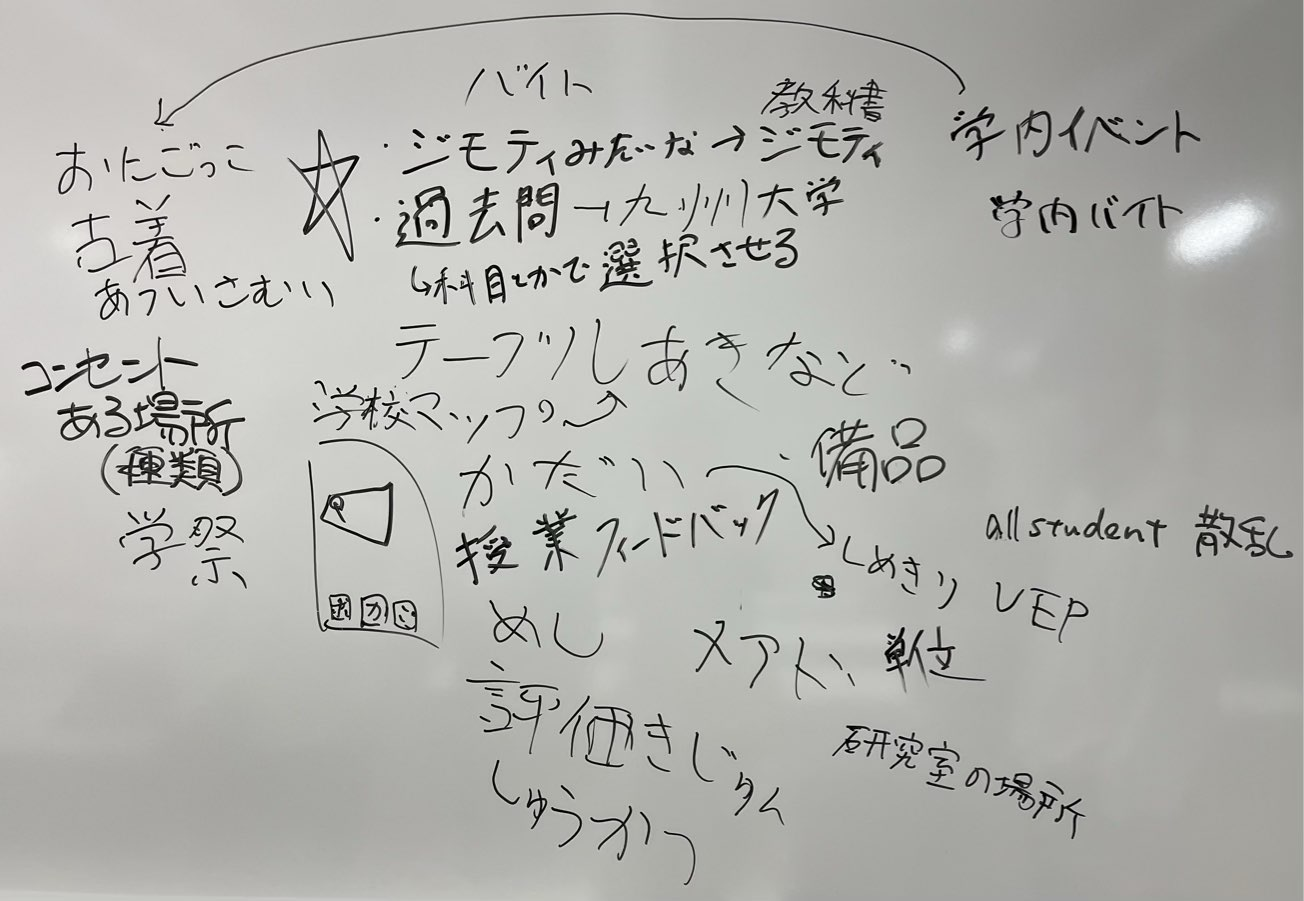
\includegraphics[width=8cm]{images/2.2_whiteboard.jpg}
    \caption{ホワイトボードの板書}
    \figlab{brain}
\end{figure}

\bunseki{大須賀雅也}

\section{フィールドワーク}

学内での問題点をより明白化するために，すでに自分たちで推測した問題点を意識して大学内を歩き回った．空き教室や空きテーブルをわざわざ歩いて探す必要があったり，コンセントも実際に行かないとあるか分からないのが現状だった．また，情報集めの一環として周りの友人に話を聞いた．大学に対する不満や問題点，現在検討中のアイディアへの意見，どんな機能があったら良いかなどを質問した．検討中のアイディアとしては，空きテーブルの情報，教科書などを受け渡すコミュニティや情報をまとめるなどがある．学生の不満点として共通していたのは，情報の集めづらさであった．HOPEやSTUDENTSといった各サイトに情報が散らばっていたり，書いている情報が違っているという状況に困惑している学生が多かった．また，検討中のアイディアに対して，絶対に必要な機能というわけではないが，あればとても便利になるという意見が多く，公立はこだて未来大学の問題点を再認識することができた．

\bunseki{齊藤輝}


\section{プロダクトの決定}

6月2日に公立はこだて未来大学で使えるアプリという案の問題点と新たなプロダクト案に関するブレインストーミングを行った．授業の課題などの科目情報，その他の学校に関することなど分散した情報を統合したいと話し合ったが，情報を取得する技術をどうするかが議題となった．科目によって課題の公開の仕方は別々であるため，API取得といった技術を使用する必要があるが，現状可能なのか分からなかったため，卒業研究で同じ分野に取り組んでいる方に話を聞いた．現在オープンデータを作っていて時間がかかるため待つしかないとのことなので，他のアイディアを深掘りすることにした．TAの方が，「まずはとにかくアイディアを出したほうが良い」と仰っていた．そのため，実際にアプリで何をしたいかホワイトボードに書き出した．どのような機能があって誰が対象なのか，何を解決できるかなどを話し合った．また，そのアイディアが実現可能なのかその都度担当教員に確認しながら進めた．最終的に，空き教室なども分かる学内のマップ，過去問，科目情報やその他の情報，教科書などを受け渡すコミュニティの機能を揃えたアプリを作成することに決定した．

\bunseki{齊藤輝}

\section{既存サービスの調査}

私達は6月7日に既存のサービスがないか調査を行った．その結果，「九州大学（非公式）\footnote{https://apps.apple.com/jp/app/九州大学-非公式/id158535402}\footnote{https://play.google.com/store/apps/details?id=com.kaede.KyushuUniversity}」「東海大学　スクールアプリ\footnote{https://apps.apple.com/jp/app/東海大学-スクールアプリ/id610479211}\footnote{https://play.google.com/store/apps/details?id=jp.co.disc.schoolnavi.dhdeijj}」などがあることがわかった．これらのアプリは，学生証，大学のホームページと連携したニュース，アプリのレビュー，時間割，学校生活についての情報などの機能を有していることがわかった．既存のアプリケーションでは空き教室や空きテーブルやコンセントの位置情報を提供しているものはない．既存のアプリケーションでは自分たちが必要としている機能には対応していない．また学生同士が教科書の受け渡しをするコミュニティの提供もない．学生はキャンパス内の施設やイベント，サービスに関する情報をパソコンからではなく手元にあるモバイル端末から簡単に入手できる．また公立はこだて未来大学ではWebアプリとして，着席QRコード読み取りを便利にするスマートフォン向けアプリケーションRALAF\footnote{https://fun-dev.github.io/RALAF/}（ららふ）がリリースされており，コロナ禍における教室での着席にQRコードによる学内での入退室着座登録を行っていた．

\bunseki{高橋慧流}

\section{技術検証}

私達は6月7日に奥野教授から大学の時間割情報を取得できるAPIについての話を頂いた．さらにTAの方から6月9日にOpenDBと実装状況についての説明を頂いた．OpenDBとは公立はこだて未来大学の教務システムのデータをAPIで提供するシステムである．実際には教務システムとOpenDBのデータベースは別であり，毎日0時に教務システムのデータベースからOpenDBのデータベースにコピーするパッチが実行される．7月18日現在，OpenDBでは主に時間割情報を取得できる．時間割情報として，時間割，教室，教室変更，休講，補講があり，時間割曜時（開講される曜日時限），時間割副担当教職員，時間割教室（開講される教室）は時間割に対して複数存在するため，エンティティを分割する．時間割は時間割一覧を取得するほか，時間割コードを指定すると指定された時間割を取得できる．教室は教室一覧を取得するほか，教室コードを指定すると指定された教室を取得できる．教室変更は教室変更一覧を取得できる．休講は休講一覧を取得できる．補講は補講一覧を取得できる．時間割曜時は，時間割コードを指定するとその時間割の開講曜日と時限が複数取得できる．時間割副担当教職員は，時間割コードを指定するとその時間割の副担当教員を複数取得できる．時間割教室は，時間割コードを指定すると教室コードを複数取得できる．
\bunseki{南川虎之介}


\section{プロダクト名の決定}

プロダクトの機能が完全には決まっていないため，プロダクト名はまだ決定できていない．
\bunseki{鈴木利芳}

\section{対象者の明確化}

私達が開発するサービスの対象者は，公立はこだて未来大学に在籍している学生である．私達が対象者について考え始めたのは6月2日のグループワークである．私達はプロジェクト学習で開発するものは，私達自身に役に立つものにしたいという思いがあった．そういったサービスであれば問題の改善に対するモチベーションが高くなると考えたからである．そのため，私達全員が利用しているものを改善したいと考えた．その条件を満たしたうえで積極的に改善したいものを考えた結果が公立はこだて未来大学であった．こういった理由から公立はこだて未来大学に在籍している学生が対象者となった．
\bunseki{大須賀雅也}

\section{問題の明確化}

私達が最初に提起した問題は「大学のシステムが使いにくい」であった．これは私達が公立はこだて未来大学を対象にしたサービスを作ると決まった時，真っ先に挙げられた問題である．私達は，公立はこだて未来大学に在籍している学生として，日々大学が提供したシステムを利用している．公立はこだて未来大学のシステムがなぜ使いにくいのかについての意見を出し合った．その結果，HOPEやSTUDENTSの情報がまとまっていないということが分かった．ほかに提起された問題は，空き教室の情報がどこにあるのかわからないということである．授業と授業の間の空き時間に課題などを行うための空き教室を探すのが面倒で分かりにくいということである．それに付随して，空きテーブルを探すのも面倒だという意見も出た．
\bunseki{大須賀雅也}

\section{目的の明確化}

私達の当初のコンセプトは「痒いところにすぐ手が届く」というものであり，目的は「自分たちが使いやすいものを作る」というものであった．これは，実際に公立はこだて未来大学の学生として過ごして，情報が分散していたり，空き教室を探すことが大変であるといった問題点を自分たちで実感し，この問題をもとに決めた目的である．\par
一度この内容で中間発表用のスライドに記述したところ，奥野教授から，「作ることが目的になっていないか」というフィードバックを頂いた．このフィードバックをもとにグループメンバー全体で改めて目的として適切であるか話し合ったところ，もっと具体的な結果を含む内容にしたいという考えに至った．この目的は，何を作りたいのかも分からない曖昧な内容になってしまっていた．理想の目的は，背景となった問題点を解決することであり，その内容を含む内容にしたいと考えた．最終的には，「未来大の情報をまとめたアプリを作り利便性を高めたい」という目的に決定することにした．
\bunseki{齊藤輝}

\section{ヒアリング}

中間発表後の質疑応答の時間を利用して,アプリに欲しい機能があるか聞いた.案として,車の相乗り機能や先輩方の科目のフィードバック機能,サークル情報,院試情報などが挙げられた.

\bunseki{齊藤輝}

\section{中間発表}
\subsection{準備}
中間発表はプロジェクト間での交流を目的とし，それに向けてプロジェクトの内容を紹介するメインポスター，スライド，スピーカーノートを作成した．中間発表の準備は6月16日から開始した．スライドやスピーカーノートは担当教員やTAの方々にレビューを依頼し，何度も内容を修正した．スライドの作成ではスライドの構成とスピーカーノートについて，齊藤がまとめ，修正した．スピーカーノートでは発表の規定時間に収まるように注意して作成し，中間発表では前半と後半に分かれているため，発表者が異なるため，発表内容に違いが現れないように注意した．

\bunseki{高橋慧流}

\subsection{中間発表会}
中間発表は，7月10日の15時20分に対面で行われた．発表は前半と後半に分かれており，どちらも15分3セットで進行された．最初の10分は，事前に作成したスライドを使用して，本プロジェクトと3つのグループについて紹介した．その後，5分間は質疑応答の時間が設けられた．本プロジェクトの発表形式は，全体の説明をする発表者1名と各グループの発表者1名の合計4名で行われた．
\begin{figure}[H]
    \centering
    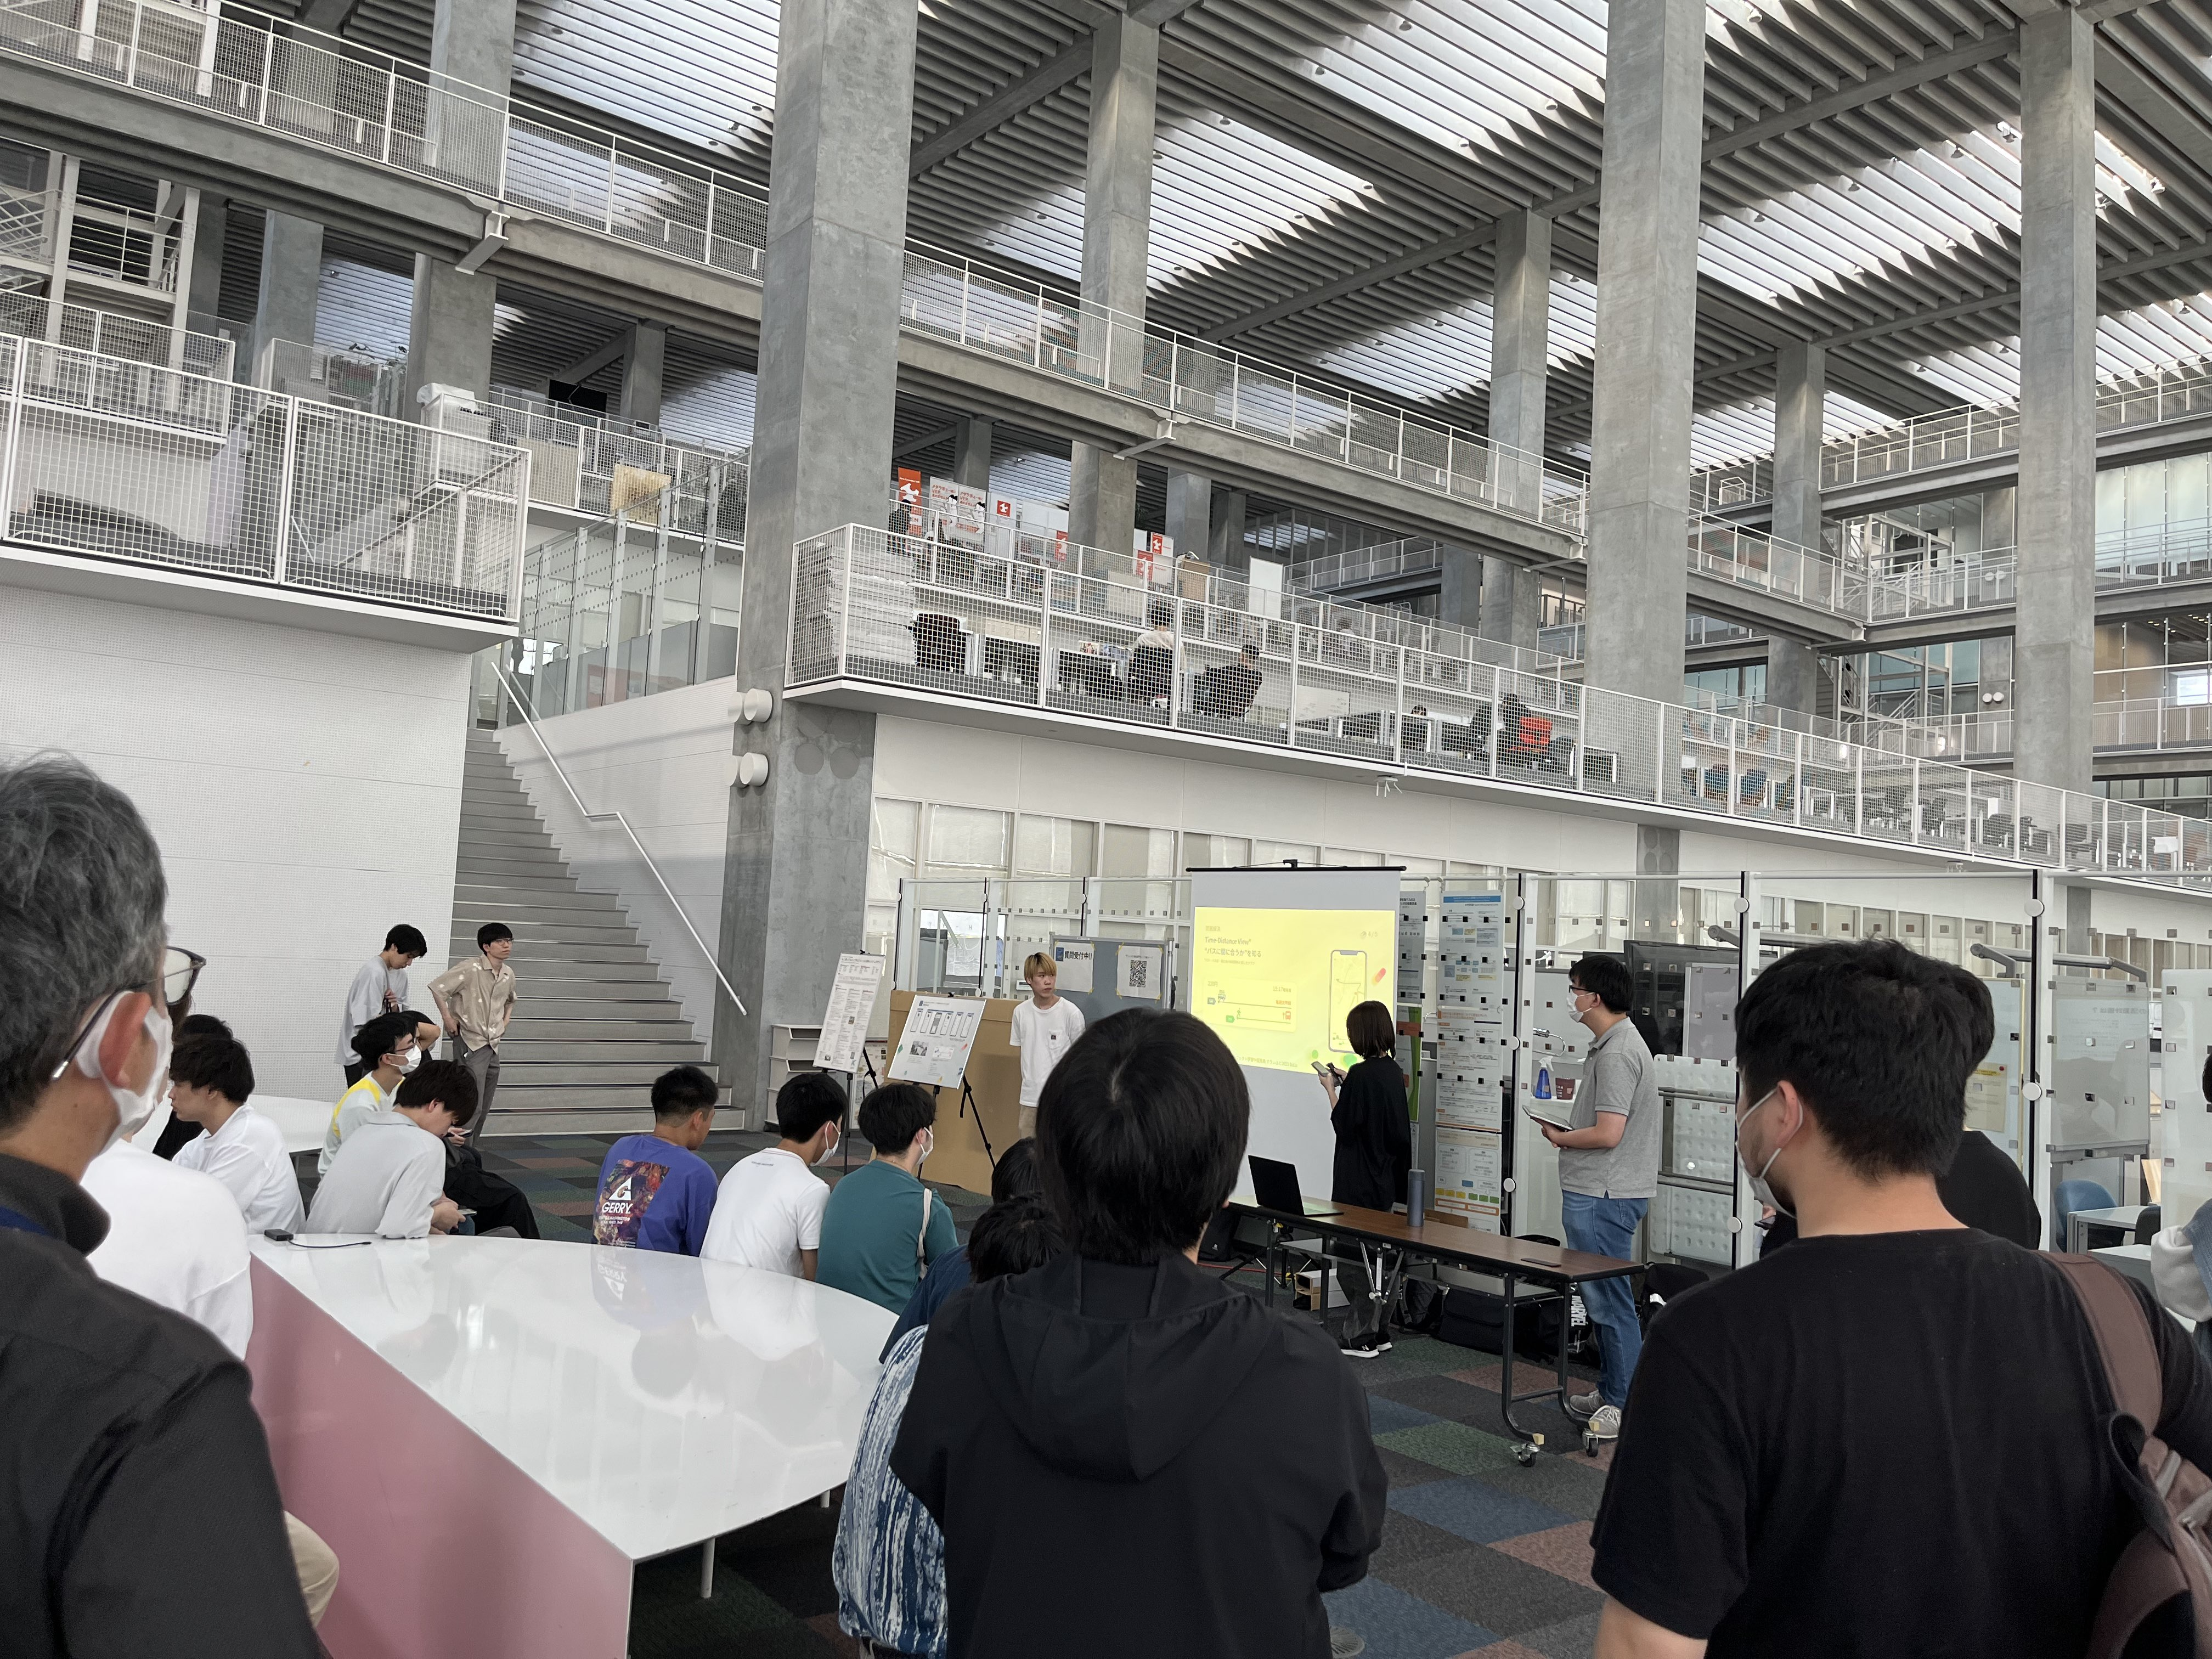
\includegraphics[width=8cm]{images/presen.jpg}
    \caption{中間発表の様子}
    \figlab{tyuukann}
\end{figure}
\bunseki{高橋慧流}

\subsection{フィードバック}
中間発表では，先生方や学生から主にアプリの機能案に関するフィードバックをいただいた．特に，「どこから情報をもってくるのか」という指摘が多くあった．このフィードバックは，アプリの要件定義において重要な視点となり，今後の開発に活かすことができる．また，以下はいただいた具体的なフィードバックである．
\begin{itemize}
      \item HOPEのAPIを使用できるのか
      \item なぜアプリに拘るのか
\end{itemize}
さらに，アイディアとしては以下のものが提案された．
\begin{itemize}
      \item 学生同士の車の相乗り募集
      \item 学生による科目のフィードバック
\end{itemize}

車の相乗りでは特に冬季においてバスが混雑し，相乗りができれば便利だというニーズがある．課題としては，情報の漏れや網羅性の確保が求められる．HOPEの拡張機能でも実現可能ではないかとの提案もあった．科目のフィードバックでは楽単情報やサークル情報，院試情報など，学生間での科目に関する情報共有やフィードバックが重要であるとされた．これらのフィードバックは，アプリのユーザーのニーズや期待に応えるために，フィードバックを踏まえながらアプリの機能や特徴を明確化していきたい．

\bunseki{高橋慧流}

\section{機能の考案}
6月2日にブレインストーミングを用いて考えた．ブレインストーミングでホワイトボードに機能案を書いた（図\ref{fig:kinou}）.その後，その中から学生生活に必要かどうかをメンバーで審議し，必要な機能を絞った．そして機能として大まかに四つの分類に振り分けた．振り分けた内容として，情報発信，情報系，授業系，マップ系とした．情報発信については要らなくなった教科書などを交換するための場を設けることや，教員が不要なった備品を譲渡する場を設けることが挙げられた．情報系は学内で募集しているアルバイト，学内のイベント，講義の過去問，就活の情報がひとまとめに見られることなどが挙げられた．授業系は現在，授業の情報とシラバスが別々のサイトで公開されているため両方を参照するのに当たって相互性を持つようにすること，課題の締め切りを通知，学生から後輩に参考になるような授業のフィードバックアンケートの場を設けるなどが挙げられた．

\begin{figure}[H]
    \centering
    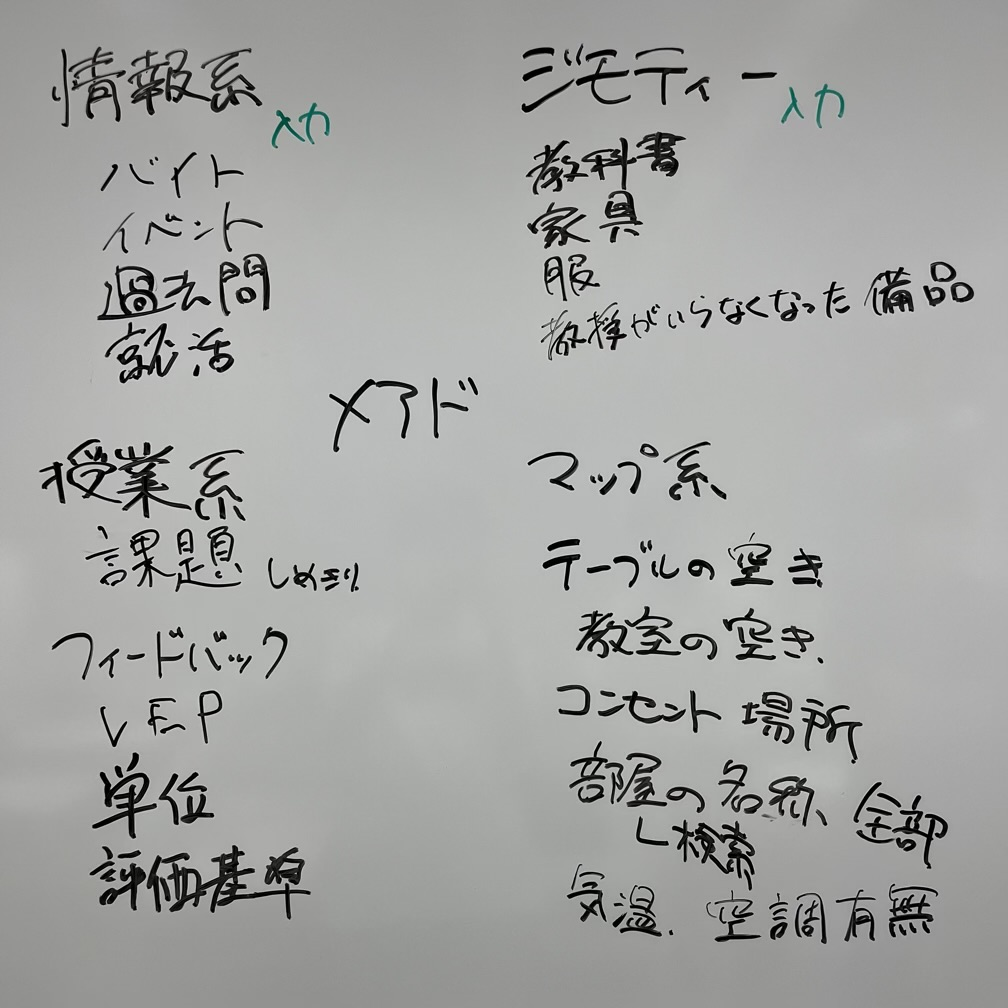
\includegraphics[width=8cm]{images/2_14.jpg}
    \caption{機能の案}
    \figlab{kinou}
\end{figure}
\bunseki{高橋慧流}

\section{プロダクト最終決定}
現時点で，プロダクトバックログの作成を行っていないため，プロダクトの最終決定を行うことはできていない．
\bunseki{鈴木利芳}
\chapter{開発するアプリケーション }

\section{目的とコンセプト}
公立はこだて未来大学での生活は不便なことが多々ある．大学が提供しているHOPEやSTUDENTSは情報が散乱していてどこにどの情報があるのかすぐにわからないという問題がある．そのため私達は，公立はこだて未来大学に在籍している学生に向けてHOPEやSTUDENTSにある情報をまとめるアプリを開発し，公立はこだて未来大学の学生が簡単に欲しい情報にアクセスできるようにすることを目的とした．そして，システムに存在する情報だけでなく，公立はこだて未来大学に在籍している学生として生活に必要な情報もまとめることで大学生活の利便性を高めることが目標である．

\bunseki{大須賀雅也}

\section{機能}
私達は，公立はこだて未来大学での生活において不便である点を考え，それらを解消できるような機能についてのアイディア出しを行った．既存の公立はこだて未来大学のシステムで使いにくい部分を解消する機能に加えて，「こんな機能があったらいいな」という機能を中心にアイディアを出した．それらに基づいて，実装を検討している機能を紹介する．
\bunseki{大須賀雅也}

\subsection{授業系の情報をまとめる機能}
この機能では，シラバスや学生の口コミなどの科目情報をまとめ，見やすく表示する．シラバスについては中間試験・期末試験の有無やレポートの有無などの成績基準の情報や，必修であるか選択であるかなどの区分を詳しく表示する．また，科目ごとに学生の口コミを投稿できるフォームを用意する．これらを表示することで，学生の履修登録時の科目選択の参考にしてもらうことを目標としている．
\bunseki{南川虎之介}

\subsection{バイトやイベントなどの情報をまとめる機能}
この機能では，学生または教員がバイト募集やイベントなどの告知をできる．これらの情報は学内メールや大学構内の掲示板，学生個人のSNSなどに分散している．これらの情報をこの機能内で投稿してもらい，ユーザがこの機能だけで情報を収集できるようにする．
\bunseki{南川虎之介}

\subsection{空き教室やテーブルの情報を表示する学内マップ機能}
この機能では，空き教室やテーブルの情報を表示する学内マップを表示することができる．STUDENTSから教室の予約情報を取得し，空き教室を表示する．テーブルの情報とは，コンセントの位置や席数など，学生が席を探すうえで必要な情報を表示する．この機能により，学生が教室や席を探す際の負担を軽減し，移動にかかる時間を減らすことができる．
\bunseki{大須賀雅也}

\subsection{学生同士で不必要な物品をやり取りする機能}
この機能では，不要になったがまだ利用価値があるものを受け渡すことができる．例えば，教科書・車・家電等の受け渡しの仲介をすることで, 必要なものをお金が無くて買えない学生の経済的な負担を軽減する. 不要なものを写真や詳細付きで投稿でき, それを欲しいユーザに条件が合えば受け渡すことができる. 
\bunseki{齊藤輝}

\subsection{過去問をまとめる機能}
この機能ではユーザが中間試験や期末試験等の過去問のダウンロードやアップロードを自由にできる．コースや学年などを選択し，それにより絞り込まれた科目一覧が表示される．科目名をタップすると年度ごとの過去問が表示される．先輩との関わりがない学生をメインターゲットとしている．
\bunseki{齊藤輝}


\chapter{知識・技術習得}

\section{リスク分析}
%各人の担当課題の概要と，プロジェクト内における役割・位置づけを記述する．
プロジェクトを本格的に開始する前に，リスク分析を行った．各個人がプロジェクト活動で起こり得ると思う問題とその発生確率，発生した場合の被害，問題の対策について考えた．考えたものについてランダムに分かれたグループ内で発表し，グループ単位でGoogleスプレッドシートにまとめ，さらにそのスプレッドシートをもとに全体で1つのGoogleスプレッドシートにまとめた．その後奥野教授からフィードバックを頂き，今後の活動に役立つ共通知識を得ることができた．
\begin{figure}[H]
    \centering
    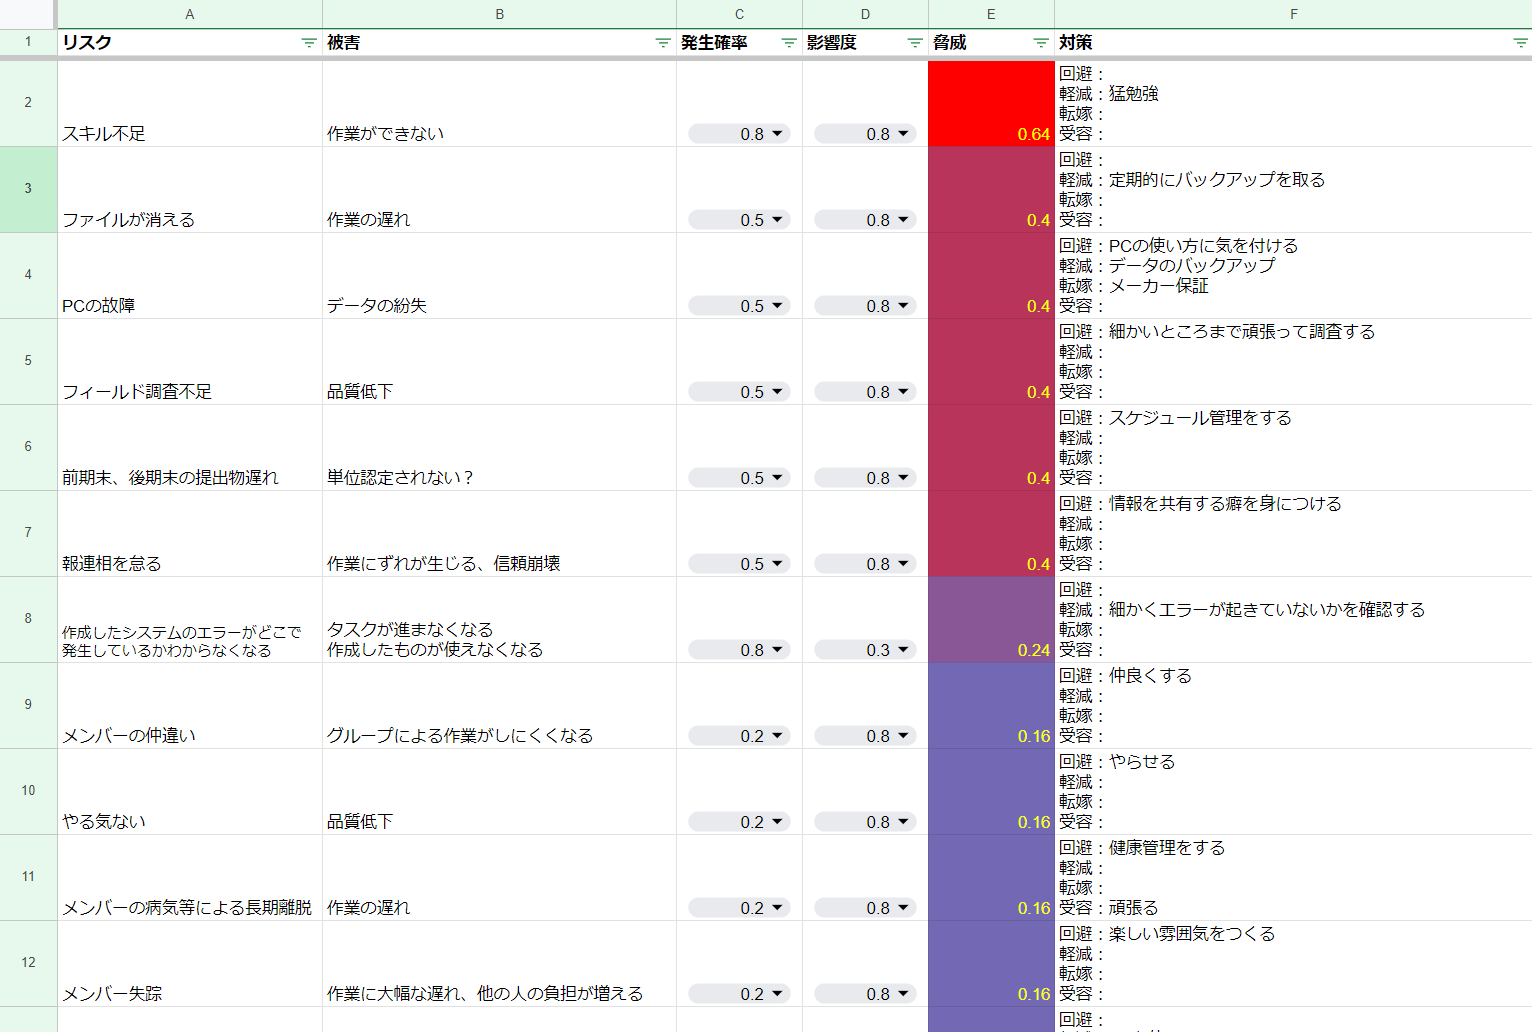
\includegraphics[width=12cm]{images/4.1_risk.png}
    \caption{リスク分析の抜粋}
    \figlab{risk}
\end{figure}
\bunseki{大須賀雅也}

\section{アジャイル開発概論 （enPiT e-Learning）}
プロジェクトの開始時に事前ビデオ教材「アジャイル開発概論（enPiT e-Learning）」の「プロジェクト学習のためのプロジェクトマネジメントの基礎」を視聴した．この学習を通じて，アジャイル開発の概念と原則について詳しく学んだ．プロジェクトマネジメントについては，プロジェクトを計画し，進行させるための方法論で，プロジェクト内での役割について学び，プロジェクトの成功に向けて必要な活動に取り組むことが重要である．具体的に，計画立案，リスク分析，スケジュール管理などの内容について詳細に学んだ．これらの知識を身につけることで，今後のプロジェクト学習活動において不可欠なスキルを獲得し，メンバー全員が共通の知識を持つことで，グループ活動を円滑に進めることが可能である．
\bunseki{高橋慧流}

\section{フィールドワーク入門講座}
フィールドワークがどのような活動なのか理解するため，5月31日に南部准教授と元木准教授による対面でのフィールドワーク入門講座を，プロジェクトメンバー全員で受講した．講座はスライド（図\ref{fig:field}）を用いて，そもそもフィールドワークとはなにか，実際に過去のフィールドワークではどのようなことを行い，どのような問題が発生したか，何に気をつけるべきか（注意事項）を教えていただいた．実際に現場に行って問題点や解決の糸口を見つけることの重要さや，ただ街をぶらぶらするのではなく社会や文化を知るために観察と記録を怠らないことが大事であるということを学んだ．
\begin{figure}[H]
    \centering
    \fbox{
    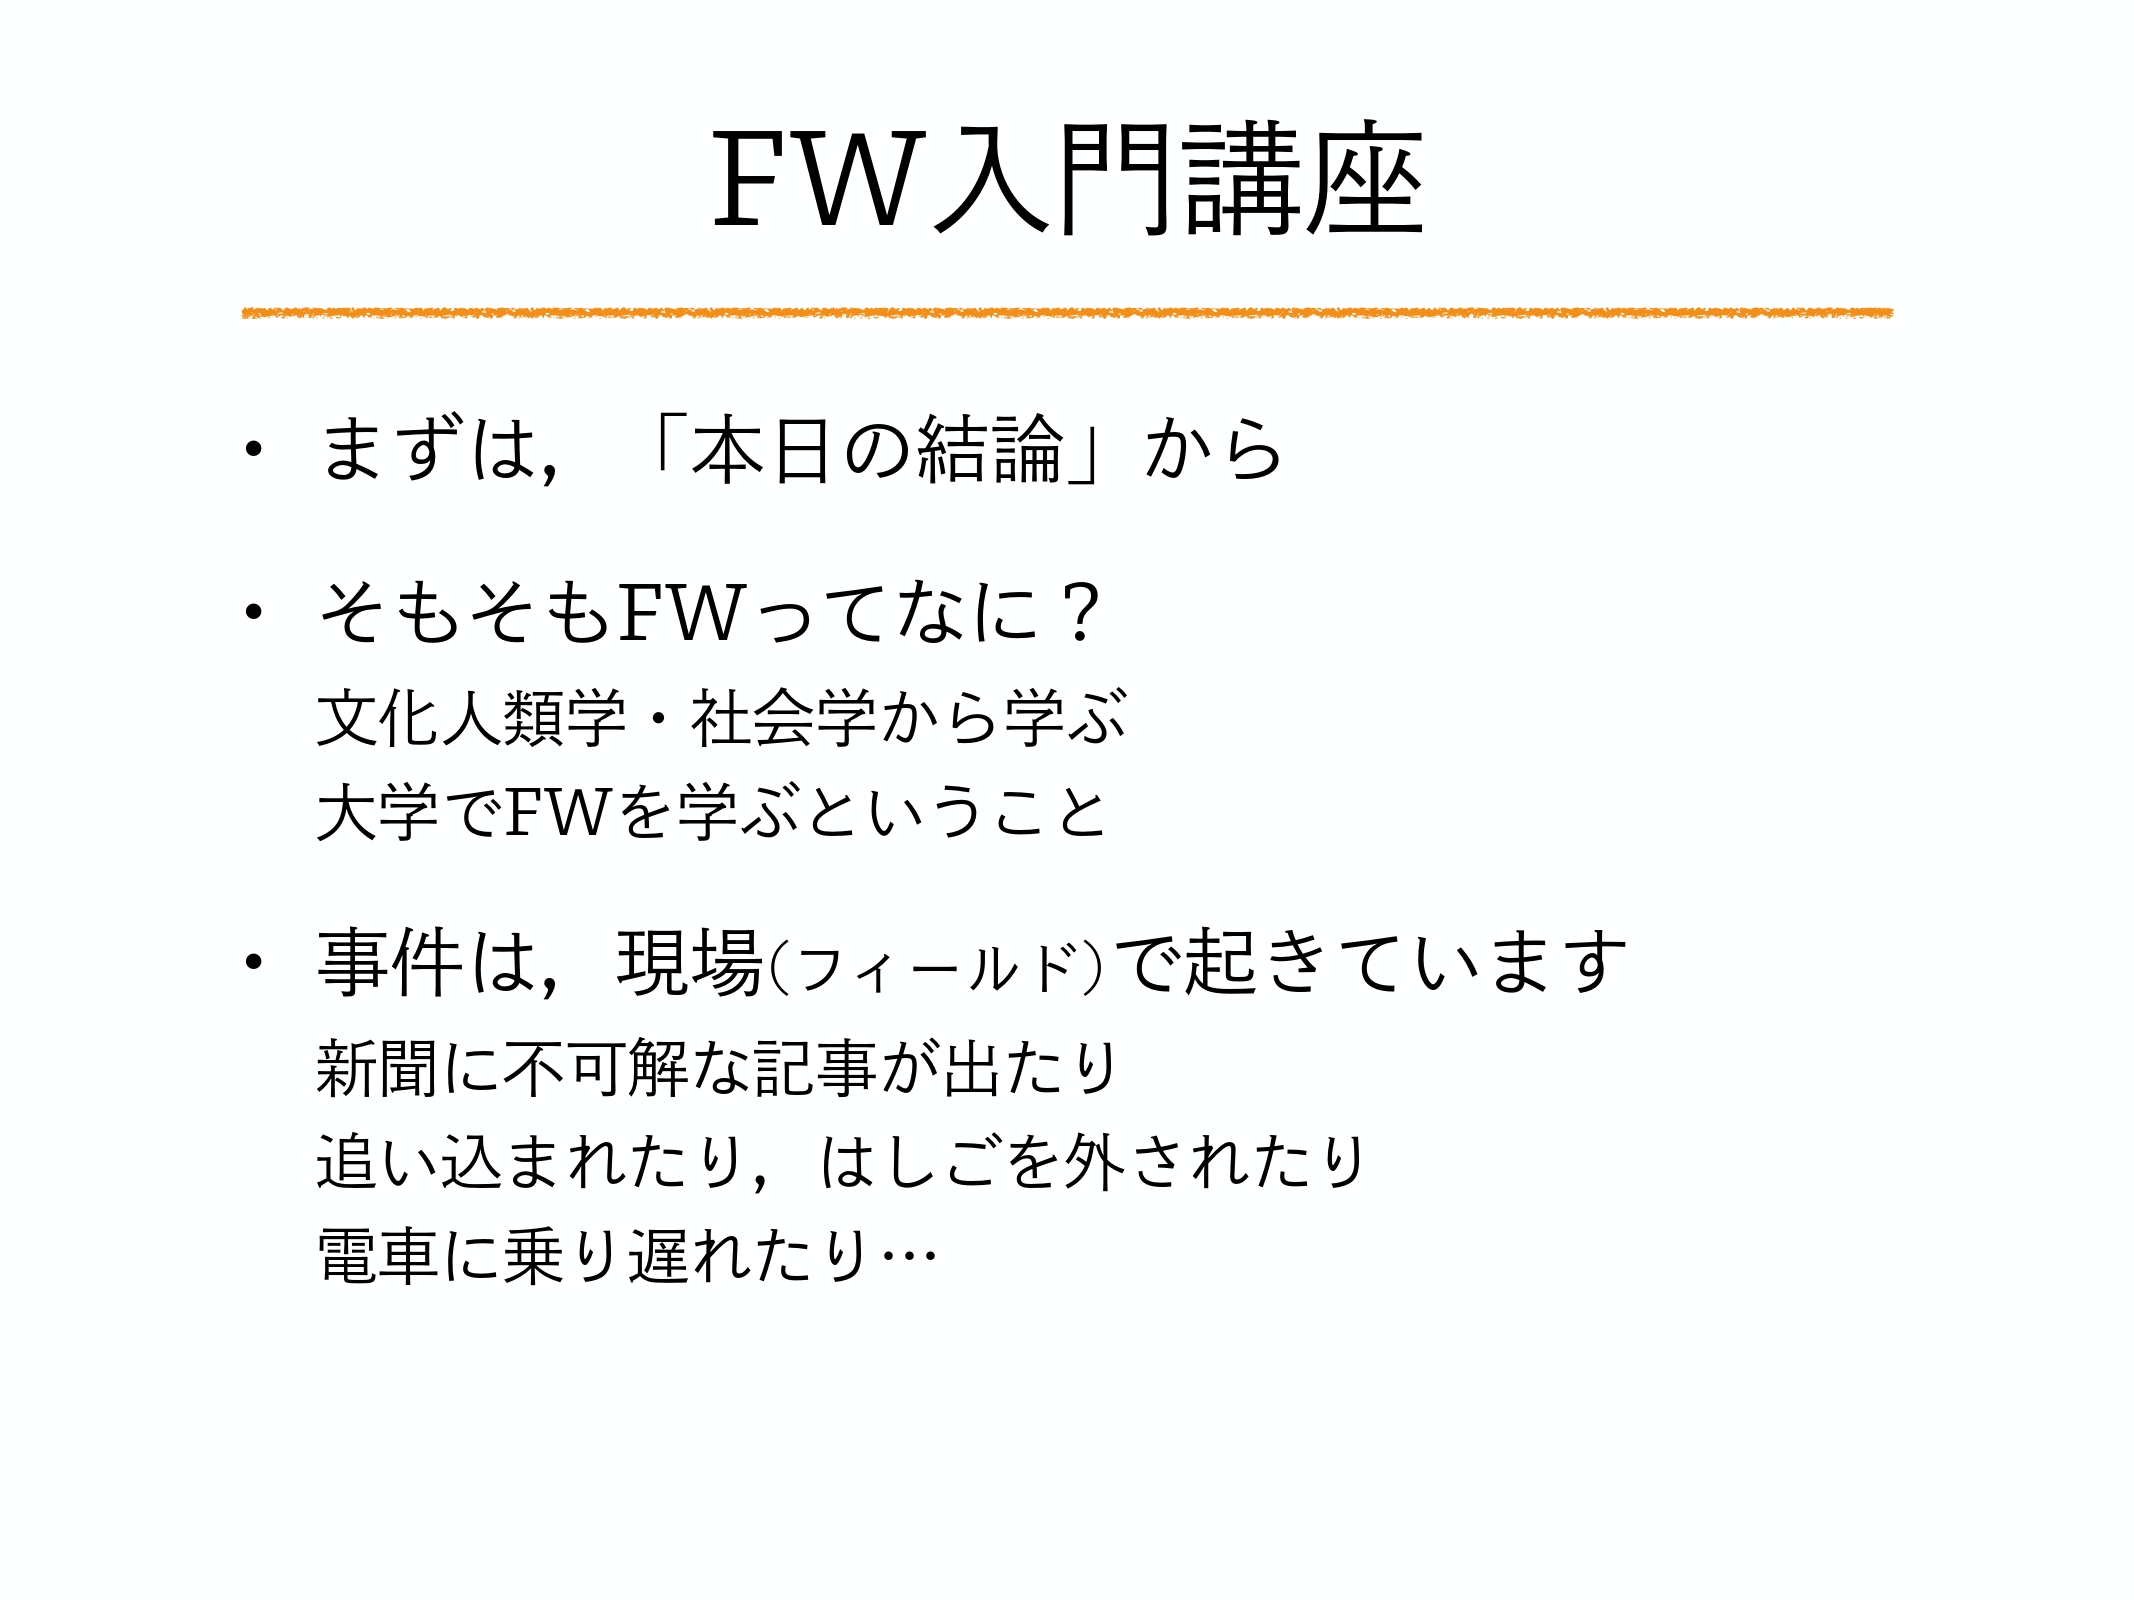
\includegraphics[width=8cm]{images/fieldwork.jpg}
    }
    \caption{フィールドワーク入門講座\cite{field}のスライドの一部}
    \figlab{field}
\end{figure}
\bunseki{齊藤輝}

\section{アジャイルワークショップ}

\subsection{DNPアジャイルワークショップ}
私達は5月29日に開催された大日本印刷株式会社主催のDNPアジャイルワークショップに参加した．大日本印刷株式会社が開発したアジャイル開発の流れについてがわかるボードゲームを学生同士で体験し，アジャイル開発とスクラムに関する知見を深めることができた．特に知識や技術を先に習得しておくことは後の開発をスムーズに進めることになり，非常に重要であることがわかった．
\bunseki{南川虎之介}

\subsection{アジャイルワークショップ}
私達は6月14日に株式会社アトラクタの永瀬美穂氏を講師に迎えて，アジャイルワークショップをプロジェクトメンバー全員で受講した．このワークショップでは，アジャイル開発についての知識をさらに深める機会を得た．ワークショップの前半では，ビデオ教材の内容をより詳しく学ぶためのレクチャーが行われた．アジャイル開発の原則や手法について，具体的な事例を通じて理解を深めることができた．これにより，アジャイル開発がどのように実践されるのか，どのようなメンバーの役割分担があるのか，プロジェクトの進行方法などについてより具体的な理解が深まった．ワークショップの後半では，前半で学んだ知識を活かして，オンラインの投票サービス「Mentimeter」を用いたクイズ大会が行われた．このクイズ大会を通じて，実際のプロジェクトシナリオに基づいた問題に対し，アジャイル開発の手法やアプローチを適用しながら解答する経験をした．これにより，アジャイル開発が具体的なプロジェクトにどのように適用されるのかを実践的に学ぶことができた．
\begin{figure}[H]
    \centering
    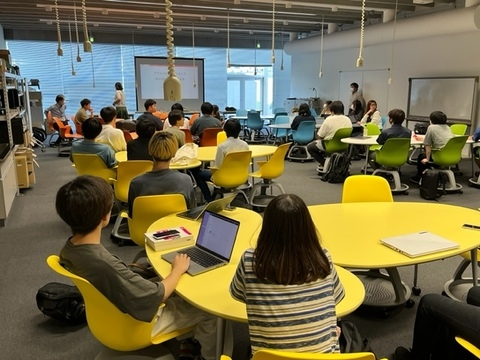
\includegraphics[width=8cm]{images/4.4.2_agilews.jpg}
    \caption{アジャイルワークショップの様子}
    \figlab{agilews}
\end{figure}
\bunseki{高橋慧流}

\section{GitHub勉強会}
私達はグループ内でGitHubの勉強会を行った．コミットやプッシュ，プル，フェッチなどの操作やリポジトリやブランチなどの用語についての知識を得た．また，危険な操作やエラーの対処法についてを学んだ．その後各自リポジトリを作成し，テスト用のFlutterプロジェクトでコミットやプッシュ，プルなどの基本的な操作を実践した．
\bunseki{南川虎之介}

\section{SCRUM BOOT CAMP THE BOOK スクラムチームではじめるアジャイル開発}
伊藤恵教授から書籍\wasyo{SCRUM BOOT CAMP THE BOOK スクラムチームではじめるアジャイル開発}\cite{scrumb}を借りた．この書籍はアジャイル開発について詳しく解説されており，時間があるときに読んで学んだ．特にスクラムというアジャイル開発の手法に焦点を当てている．本書を通じて，スクラムの基本的な役割であるプロダクトオーナーやスクラムマスターの役割や責任について理解を深めた．彼らの役割は，プロジェクトの成功に欠かせないものであり，それぞれがチームの効率性と成果の最大化を担っている．また，スクラムの始め方や見積もりの方法についても学んだ．スクラムでは，プロジェクトの開始時に適切なフレームワークを設定し，効果的なスプリントの計画と実行を行う．見積もりは，タスクの時間的な所要量を適切に評価するための重要なスキルであり，正確な見積もりを行うことでスプリントの進行管理が円滑になる．

\bunseki{高橋慧流}

\section{Flutter}
Flutter\footnote{https://flutter.dev}は，2018年にGoogleが正式リリースしたオープンソースのフレームワークである．Flutterが備える最大の特徴は，「iOSとAndroidのアプリを一度に開発できる」という点が挙げられる．加えて，Flutterは，ホットリロードに対応しているため高速開発が可能である．これらの理由から，Flutterによる開発を行っていくことに決めた．
\bunseki{南川虎之介}

\section{Firebase勉強会}
Firebase\footnote{https://firebase.google.com}勉強会はグループ内で夏季休暇で実施する予定である．
\bunseki{南川虎之介}

\section{API勉強会}
API勉強会はグループ内で夏季休暇で実施する予定である．
\bunseki{南川虎之介}

\chapter{学び}

\section{共通認識の重要さ}
本グループでは，プロダクトのテーマ決めから現在に至るまで，メンバー全員で共通認識を持つことを重要視してきた．伊藤恵教授から貸して頂いた書籍\wasyo{SCRUMMASTER THE BOOK 優れたスクラムマスターになるための極意――メタスキル，学習，心理，リーダーシップ}\cite{scrumm}に書かれていた通り，グループメンバー全員がプロダクトのターゲットや目的に対し共通認識を持つことは開発を進めるにあたって必要不可欠であるため，これらについて優先的に話し合ってきた．また，チームメンバーそれぞれの役割についても認識のずれが生じないよう全員で確認し合った．これによって，開発や中間発表の提出物作成を円滑に進めることができた．今後の開発においても，グループメンバー間で認識にずれがあった場合，プロダクトに支障をきたすため，細かなことでも，共通認識を持つことは重要であると考える．


\bunseki{鈴木利芳}

\section{議事録の重要さ}
本グループでは，何をどのように決定し，いつ何が決定されたかを後から確認できるよう議事録をとりながら活動を進めた．議事録は，決定した内容や過程だけでなく，決定に至るまでの思考や発言も記録する必要があるため，多くの肉体的コストがかかるが，それを上回るメリットがあることを学んだ．特に，報告書やポスター，発表スライドの作成の際は，議事録を見直すことで作業をスムーズに進めることができ，メリットを享受することができた．また，議事録に，次週の活動方針や次週までに達成したい目標を記録することで，グループメンバーがそれぞれ何をやらなければいけないのかが明確になった．これにより，開発をスムーズに行えるだけでなく，グループメンバーの共通認識を明確にすることができた．議事録は，これまでの開発を振り返り，これからの活動方針を決定するためにも，必要不可欠なものであると考えられる．
\begin{figure}[H]
    \centering
    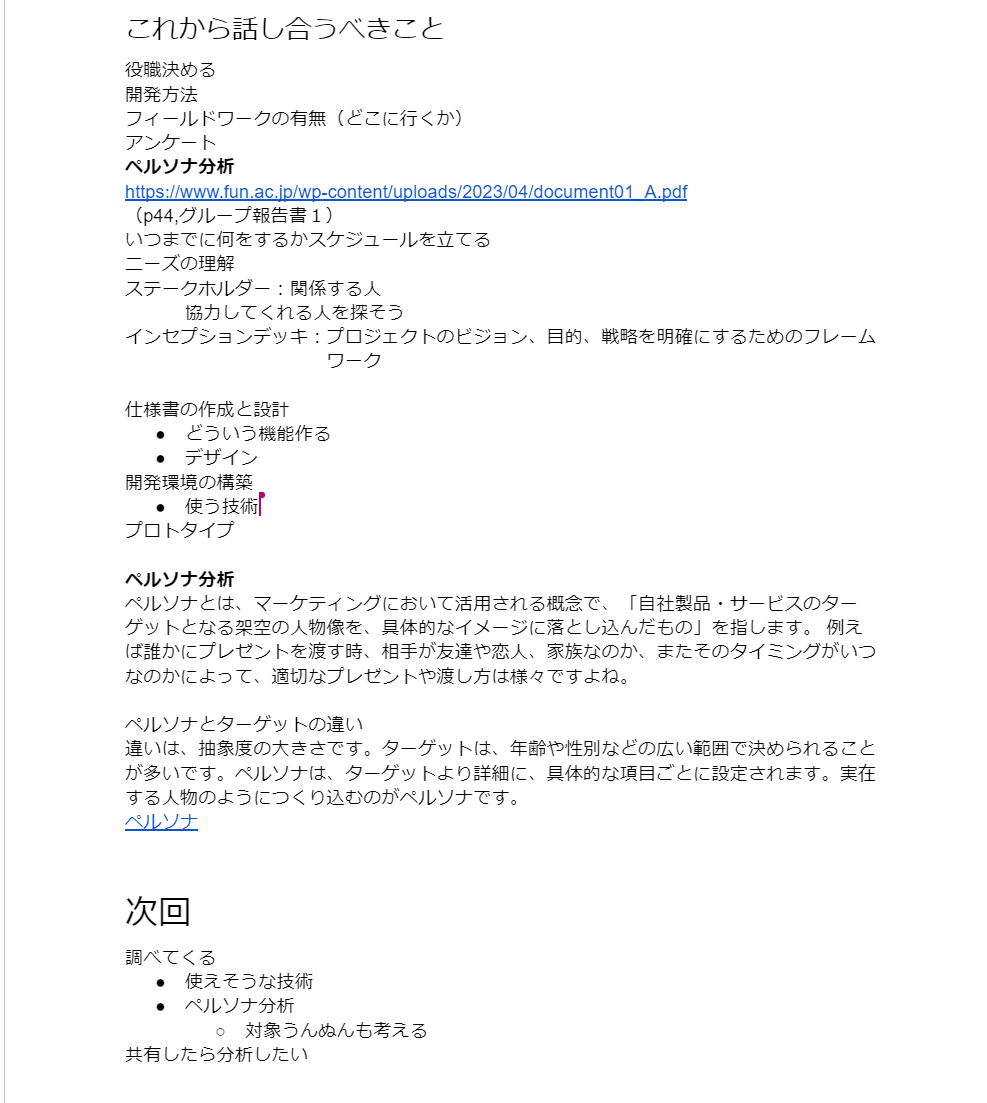
\includegraphics[height=16cm]{images/5.2_giziroku.png}
    \caption{実際の議事録の様子（一部を抜粋）}
    \label{fig:giziroku}
\end{figure}
\bunseki{鈴木利芳}

\section{コミュニケーションツール}
%各人の担当課題の成果について，成果によってどのように上述した課題が解決されたか， 要求された役割は果たせたか，残された問題点はあるかを記述する．

\subsection{Discord}
プロジェクト時間外の活動で話し合いを行うためにDiscord\footnote{https://discord.com}を利用した．Discordとは，アメリカ発祥のチャットサービスである．Discordはオンラインゲームをしながら，世界中の人々とコミュニケーションをとるために生まれたサービスであるが，最近では，さまざまなコミュニティで利用されている．私達は，遠隔でも作業を効率よく進めるためにボイスチャットや画面共有機能を使用した．ボイスチャットや画面共有を使うことで，現在行っている作業の何に困っているかが明確になったことや，すぐに意見を求めたり意見を言ったりすることができた．
\bunseki{南川虎之介}

\subsection{Slack}
プロジェクト活動の進捗報告や連絡事項などを補助するツールとしてSlack\footnote{https://slack.com}を利用した．Slackとは，チャンネルベースで行われるビジネス用のメッセージングアプリである．一般的にSlackはグループコミュニケーションツールとして使われている．このツールを使うことで，メンバーが1つの場所に集まり，グループが一体となって働くことができた．
\bunseki{齊藤輝}

\subsection{ホワイトボード}
グループ活動で話し合うときは，主にホワイトボードを用いて活動していた．ホワイトボードを使う場面のほとんどはブレインストーミングを行うときである．グループメンバーの意見やホワイトボードにすべて書くことで思考を発散させた．これにより，プロダクト案プロダクトの対象者などを明確にする一助になったため，何かに行き詰まって困ったときは，ホワイトボードでブレインストーミングを行うことがいいということを学んだ．
\bunseki{斎藤輝}

\section{Figma}
Figma\footnote{https://www.figma.com}とは，ブラウザ上で動作し，デザインの作成，共有を簡単に行うことができるツールである．複数人同時での編集や閲覧が可能であるため，本開発で使用することにした．本開発では，プロダクトのUIデザインやプロトタイプの作成に使用した．
\bunseki{鈴木利芳}

\section{Git/GitHub}
Git\footnote{https://git-scm.com}とは，ソースコードの変更を保存，追跡するための分散型バージョン管理システムである．GitHub\footnote{https://github.com}とは，Gitを用いてクラウド上でバージョン管理をすることができるWebサービスである．複数のユーザーと共有し，共同作業を行うことができる．
\bunseki{南川虎之介}




\chapter{今後の活動}
本グループは，12月の成果発表までにプロダクトを完成させ，対象者（未来大生）に1回以上レビューを頂くことを目標としている．そのための今後の予定として，まず中間発表の際に，機能案やUIに関するアンケートを実施する．そのアンケート結果をもとに，プロダクトの機能の詳細を決定していく．現段階で，開発言語やプラットフォームが決定しているため，夏休み終了までは，開発に必要な技術の習得を行う予定である．また，9月には開発言語の習得と並行してUCDワークショップに参加し，人間中心設計について学び，プロダクトのデザインに役立てたいと考えている．10月，11月はプロダクトの開発を進めるとともに，レビュー及び発表に向けた準備を行う予定である．

\bunseki{鈴木利芳}


% 以降，付録(付属資料)であることを示す
\begin{appendix}



\chapter{活用した講義} 
本グループがプロジェクト学習を行っていく上で，活用した講義は以下である．
\vskip\baselineskip
ソフトウェア設計論 I\par
ソフトウェア設計論 I ではリスク分析やリスク対策の種類などについて学んでいたため,この講義で使用されていた資料を再確認するなどして活用した.
\vskip\baselineskip
ヒューマンインタフェース\par
ヒューマンインタフェースの講義でアンケートの作成方法について紹介されていたため,この講義をもとに,アンケートを作成した.


%付録の終わり
\end{appendix}

%======================================================================
%\backmatter

% 参考文献
\begin{thebibliography}{3}
\bibitem{scrumb} 西村 直人， 永瀬 美穂， 吉羽 龍太郎. \qq{SCRUM BOOT CAMP THE BOOK スクラムグループではじめるアジャイル開発}. 株式会社 翔泳社. 2020.
\bibitem{field} 南部 美砂子．\qq{フィールドワーク入門講座 for PBL 2023年度版}． https://drive.google.com/file/d/1H6-Iepfufk80NmRY0DlYInMgRa-5zOrA/view （2023年7月14日 アクセス）
\bibitem{scrumm} Zuzana Sochova. \qq{SCRUMMASTER THE BOOK 優れたスクラムマスターになるための極意――メタスキル，学習，心理，リーダーシップ}. 株式会社 翔泳社. 2020.

\end{thebibliography}

\end{document}